\documentclass[a4paper]{article}

\usepackage[brazil]{babel}
\usepackage[utf8]{inputenc}
\usepackage{amsmath,amsfonts,amssymb,latexsym,mathrsfs,amsthm,amstext,bezier,amscd}
\usepackage{graphicx}
\usepackage{indentfirst}

\begin{document}
\thispagestyle{empty}

\begin{titlepage}
	\vfill
	\begin{center}
		\parbox{6cm}{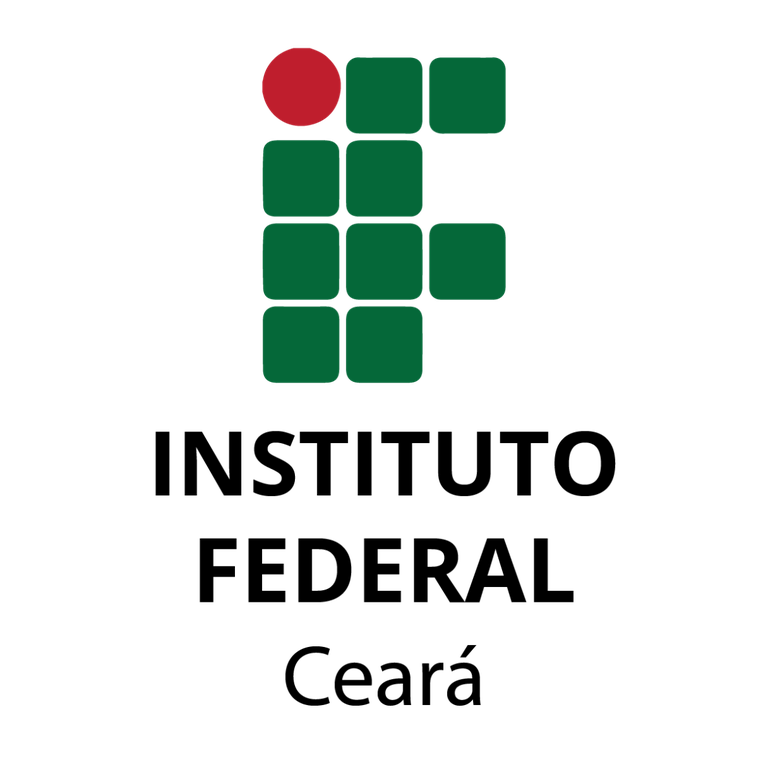
\includegraphics[scale=0.2]{logo.png}}\\
		\begingroup
		\fontsize{12pt}{0pt}\selectfont
		{\large \textbf{INSTITUTO FEDERAL DE EDUCAÇÃO, CIÊNCIA E TECNOLOGIA DO CEARÁ}}\\[0.2cm]
		\fontsize{12pt}{0pt}\selectfont
		{\large \textbf{IFCE CAMPUS MARACANAÚ}}\\[0.2cm]
		\fontsize{12pt}{0pt}\selectfont	
		{\large \textbf{BACHARELADO EM CIÊNCIA DA COMPUTAÇÃO}}\\[4cm]
		\fontsize{12pt}{0pt}\selectfont
		{\large \textbf{THIAGO MAGALHÃES FURTADO}}\\[3.5cm]
		\fontsize{12pt}{0pt}\selectfont
		{\large \textbf{Avaliação de Acessibilidade em Portais de Notícias}}\\[3.5cm]
		\fontsize{12pt}{0pt}\selectfont
		{\large \textbf{MARACANAÚ}}\\[0.2cm]
		\fontsize{12pt}{0pt}\selectfont
		{\large \textbf{2021}}
		\endgroup
	\end{center}
\end{titlepage}

\begin{titlepage}
	\vfill
	\begin{center}
		\fontsize{12pt}{0pt}\selectfont
		{\large \textbf{THIAGO MAGALHÃES FURTADO}} \\[2.5cm]
		\fontsize{12pt}{0pt}\selectfont
		{\large \textbf{Avaliação de Acessibilidade em Portais de Notícias}}\\[3cm]
		
		\hspace{.45\textwidth} %posiciona a minipage
		\begin{minipage}{.5\textwidth}
			\large Trabalho de Conclusão de Curso apresentado ao curso de Bacharelado em Ciência da Computação do Instituto Federal de Educação, Ciência e Tecnologia do Ceará (IFCE) - Campus Maracanaú, como requisito parcial para obtenção do Título de Bacharel em Ciência da Computação.\\[1cm]
			Prof. Dr. Otávio Alcântara de Lima Junior.
		\end{minipage}
		\vfill
		\vspace{2cm}		
		\large \textbf{Maracanaú - CE}
		
		\large \textbf{2021}
	\end{center}
\end{titlepage}

\begin{titlepage}
	\begin{center}
		\tableofcontents
	\end{center}
\end{titlepage}
\begin{titlepage}
\section{Introdução}
\fontsize{12pt}{0pt}\selectfont
Estamos vivendo em uma época em que a tecnologia tem avançado bastante, isso é notório se nós analisarmos as duas últimas décadas do século XX e o começo do século XXI, isto é, desde os anos 80 o mundo entrou em uma nova era, conhecida como era da informação. Assim, os computadores, os meios tecnológicos e a internet têm tido um avanço significativo, fazendo com que haja um crescimento de usuários em todo o mundo, possibilitando uma prestação de serviço para a nossa sociedade e facilitando a obtenção de informação rápida.

Entretanto, segundo a Patricia Acosta-Vargas, o Luís Antônio Salvador-Ullauri e o Sérgio Luján-Moura, muitos sites não possibilitam à todos os usuários uma boa navegação, já que alguns possuem problemas para acessar os serviços oferecidos por eles, pelo simples motivo dos usuários possuírem algum tipo de deficiência, como, baixa visão, pouca adição, diminuição da capacidade motora, dentre outros. Além disso, de acordo com o site Uol, houve uma pesquisa promovida pelo movimento Web para todos em parceria com a empresa BigDataCorp e com o Núcleo de Informação e Coordenação do Brasil, na qual, menos de 1 por cento dos sites no Brasil, dentre 14 milhões de sites, são totalmente acessíveis, e, de acordo com o IBGE de 2010, aproximadamente, 24 por cento da população brasileira apresenta alguma deficiência, totalizando cerca de 45.606.048 pessoas, como mostrado na Figura 1.\\[0.5cm]

Figura 1 - Distribuição quantitativa das deficiências no Brasil, no ano de 2010.\\
\begin{center}
	\parbox{10cm}{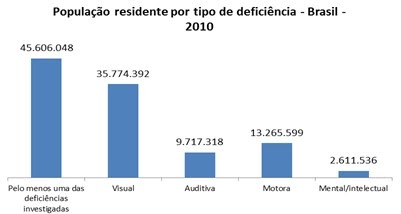
\includegraphics[scale=0.7]{IBGE-Deficiência.jpg}} \\
\end{center}

Um dos meios de sites que não são acessíveis no Brasil, são os sites de notícia, algo que é bastante inadmissível, já que eles possuem um acesso grande, segundo o site Metrópole, onde é dito que das oito plataformas digitais mais visitadas em 2020 no Brasil, três delas são de notícias, que são o globo.com, o uol.com.br e a metrópoles.com, que estão em quinto, sétimo e oitavo lugar.

Portanto, este trabalho aborda a prática do uso da acessibilidade de dez sites de notícia para pessoas que possuem algum tipo de deficiência, seja ela visual, auditiva, física ou motora, com o objetivo de analisá-los e classificá-los, como acessíveis ou não, através da análise da diretriz WCAG sobre acessibilidade, com o objetivo de incentivar todas as pessoas que estão envolvidas na formulação dessas plataformas para deixá-las cada vez mais acessíveis.

Isso será organizado durante todo o artigo da seguinte a maneira, primeiro iremos falar sobre alguns artigos publicados anteriormente sobre o assunto, mostrando em que área aconteceram os seus estudos e caracterizando a definição de acessibilidade digital por meio desse autores, mostrando o que cada um pensa sobre o assunto. Depois serão explicadas as formas de deficiência existentes que afetam a usabilidade dos sites, após isso iremos analisar a diretriz WCAG (Web Content Accessibility Guidelines), que já está na sua segunda versão, isto é, a WCAG 2.0, mostrando os princípios básicos e as recomendações para cada princípio. Além disso, apresentaremos os pontos fortes e fracos dos sites de notícias relacionado com a acessibilidade web através da análise da diretriz com o propósito de fazer sugestões de melhorias. Por fim iremos tirar conclusões sobre o que foi levantado dos devidos sites. 

\section{Revisão Bibliográfica}
Existem vários estudos e artigos que tratam sobre o tema da acessibilidade digital, artigos dos mais diversos possíveis, em várias regiões do mundo e sobre vários pontos de vista, assim iremos passar por alguns deles, mostrando qual ponto o mundo está em relação a acessibilidade web, quais pontos de melhoria são necessários nos sites em geral e quais conclusões cada autor conseguiu encontrar. 

Assim, vamos começar citando alguns artigos que definiram o significado de acessibilidade digital. O primeiro artigo escolhido foi feito aqui no Brasil, o artigo se chama "Acessibilidade digital - Uma análise em portais de Instituições Federais de Educação do Brasil", produzido pelos por esse autores em questão, o Daniel Luís Arenbardt, a Tatiane Stefanel Franchi, a Vânia Medianeira Flores Costa e a Márcia Zampieri Grohmann, no ano de 2017 usa a Organização Mundial da Saúde(OMS) para definir o termo em questão, dizendo o seguinte:\\[0.5cm]

\hspace{0.19\textwidth} %posiciona a minipage
\begin{minipage}{0.75\textwidth}
	\fontsize{10pt}{0pt}\selectfont
	O conceito mais amplamente utilizado e aceito sobre deficiência refere-se ao publicado pela Organização Mundial da Saúde (OMS), por meio de sua Classificação Internacional de Funcionalidade, Incapacidade e Saúde (CIF). De acordo com a “Convenção sobre os direitos das pessoas com deficiência”, pessoas com deficiência são aquelas que têm incapacidades físicas, mentais, intelectuais ou sensoriais a longo prazo que, em interação com diversas barreiras, podem prejudicar sua participação plena e efetiva na sociedade em igualdade de condições com os outros (Nações Unidas, 2001, p. 4).\\[0.5cm]
\end{minipage}

Então, podemos ver que, segundo esse artigo, a Organização Mundial da Saúde considera super importante o meio em que o deficiente físico está, pois o ambiente em que ele vive pode ocasionar em um impacto negativo nas suas atividades normais, pois o meio em questão poderá trazer barreiras que não podem ser ultrapassadas pelo deficiente, sejam elas físicas, sociais ou comportamentais, gerando a falta de inclusão e a falta da participação na sociedade.

Nesse artigo é mostrado que mesmo possuindo uma lei, como já foi dito anteriormente, mesmo o Brasil tendo criado o Decreto N. 5.296 de 2004 com o intuito de garantir acesso a informações em portais eletrônicos da administração pública às pessoas com deficiência, disponibilizando o Modelo de Acessibilidade em Governo Eletrônico (eMAG), principal documento de recomendações a serem seguidas para o desenvolvimento de sítios eletrônicos acessíveis a todos os usuários, e mesmo sendo sites do governo, ainda assim há um baixo uso das padronizações da acessibilidade, isso é algo bastante triste. 

No artigo foi analisado sites governamentais, no caso 107 sites de Instituições Federais de Educação do Brasil. Os pesquisadores pontuaram alguns elementos importantíssimos para a acessibilidade, dentre eles foram, atalhos de teclados, opção de alto contraste, barra de acessibilidade, existência do mapa de sítio e páginas de descrição com os recursos de acessibilidade. Além desses critérios, existem outros que não foram citados pelos artigos, como, por exemplo, ter a disponibilidade para leitores de tela, a presença de áudios e de vídeos com descrições textuais, a existência de vídeos de libras, dentre outros.

Os autores da pesquisa verificaram a existência de um grande descaso relacionado com a inclusão digital, pois apenas 14,02 por cento possuem atalhos no teclado, 22,43 por cento possuem a opção de alto contraste, 41,12 por cento possuem a barra de acessibilidade, 36,45 por cento possuem o mapa de sitio e só 14,02 por cento possuem páginas com descrições com os recursos de acessibilidade. Isso nos mostra que, segundo os pesquisadores, os resultados obtidos apontam para um elevado descaso com a inclusão digital em relação às pessoas com deficiência, de forma que o nível de adoção dos padrões de acessibilidade é extremamente baixo nos portais das Instituições Federais de Ensino.

Exitem outras diretrizes além da eMAG, como a World Wide Web(W3C), que foi criada em primeiro de outubro de 1994, no qual possui uma organização chamada World Wide Consortium, que é um consórcio com 450 membros, empresas, organizações independentes e ONGs com o objetivo de formular padrões para os desenvolvedores aos criarem os seus sites Web, esses padrões foram formulados em uma diretriz, ela é chamada de WCAG. Na citação logo abaixo do artigo “Challenges to Assess Accessibility in Higher Education Websites: A Comparative Study of Latin America Universities”, que foi produzido por Patricia Acosta-Vargas, Tania Acosta e Sérgio Luján-Moura, no ano de 2018, vemos mostra a finalidade da criação dessa diretriz e mais uma conceituação o significado de acessibilidade web:\\[0.5cm]

\hspace{0.19\textwidth} %posiciona a minipage
\begin{minipage}{0.75\textwidth}
	\fontsize{10pt}{0pt}\selectfont
	Acessibilidade na web refere-se a recursos de design da web que permitem que as pessoas percebam, entendam, operem e apoiem tecnologicamente os sites. O W3C desenvolveu as Diretrizes de Acessibilidade de Conteúdo da Web (WCAG) 2.0. O objetivo do WCAG é orientar web designers e desenvolvedores para a eliminação de erros de acessibilidade. A Acessibilidade na Web visa garantir um acesso satisfatório à Web para o máximo de pessoas, independentemente de suas limitações físicas, do ambiente ou dos dispositivos que utilizam para acessar as informações.\\[0.5cm]
\end{minipage}

Por meio desse artigo, vemos que, para os seus autores, a criação da diretriz WCAG tem uma importância muito grande, pois, caso os programadores em geral decidam seguir os seus princípios, eles tornarão as plataformas digitais existentes da Web cada vez mais acessíveis para todo e qualquer ser humano que deseja usá-lo, independente se o usuário possui ou não qualquer um dos tipos de deficiência, seja ela física, motora ou mental. Sendo assim, para eles, a acessibilidade na Web garanti um acesso à internet satisfatório, atingindo o maior número de pessoas possível, independente da existência de uma comorbidade  física, do meio em que o usuário está e do dispositivo utilizado para o acesso ao contudo existente no site.

Os autores Patricia Acosta-Vargas, Tania Acosta e Sergio Luján-Moura, tiveram como objetivo explicar o WCAG 2.0, onde essa diretriz tem como objetivo servir de apoio para os desenvolvedores ao uso da acessibilidade web. Ele inclui 12 diretrizes organizadas em quatro princípios diferentes, que são, perceptível, operável, compreensível e robusto. 

Começaremos pelo princípio perceptível, onde é dividido em três sentidos básicos usados pelo ser humano, a visão, a audição e o tato, assim, segundo a diretriz é necessário que o site forneça alternativas para os conteúdos de textos, seja aumentar a letra, seja o uso de braile ou seja a existência de áudios e símbolos, com o intuito de utilizar linguagens mais simples. Além disso, é preciso que tenha alternativas para a mídia em função do tempo, criando conteúdos que possam ser apresentados de formas diferentes, incluindo a separação do primeiro e segundo plano, sem haver a perda de informações ou mudança de prioridade, tudo isso usado para ajudar o usuário a ver e ouvir os conteúdos existente na plataforma.

O segundo princípio é o operável, que como finalidade definir métodos para a acessibilidade web, através da navegação e do uso de interfaces apropriadas para os deficientes, sendo divididas em quatro diretrizes que são, a disponibilidade de todas as funcionalidades por meio do teclado, fornece aos usuários tempo suficiente para ler, ouvir, entender e usar os conteúdos, uso de um design de conteúdo que não gera a indução de convulsões e fornece formas de ajudar os usuários a navegar pelo site, ajudando-o a encontrar conteúdos e funcionalidades dentro do site.

O terceiro princípio é o compreensível, no qual explica o modo de fazer o usuário interpretar corretamente o conteúdo da plataforma digital. Ele é descrito em três diretrizes diferentes, que são tornar o conteúdo do texto legível e compreensível, exibir as funcionalidades das páginas da web de forma previsível e o site ter mecanismos para ajudar os usuários a evitar e corrigir os erros existentes.

Já o quarto e último princípio é o robusto, isto é, o princípio leva em consideração a compatibilidade com as tecnologias atuais e futuras, com o intuito de maximizar a harmonização das páginas da web com os seus usuários com essas tais tecnologias.

Então, podemos ver que a diretriz é bem extensa e abrange quase todas as formas de acessibilidade existentes, agora, é preciso só que os programadores se propõem a seguir os quatro princípios básicos ditos anteriormente, com a meta de fazer tal atividade em seus trechos de códigos, fazendo com que todas as pessoas consigam manipular os seus sites, sem haver nenhum tipo de descriminação por partes dos programadores e dos produtores de conteúdos.

O terceiro artigo que iremos referenciar é o “A Heuristic Method to Evaluate Web Accessibility”, produzido por Patricia Acosta-Vargas, Luis Antonio Salvador-Ullauri e Sergio Juan-Mora, no ano de 2019, diz o seguinte:\\[0.5cm]

\hspace{0.19\textwidth} %posiciona a minipage
\begin{minipage}{0.75\textwidth}
	\fontsize{10pt}{0pt}\selectfont
	O termo acessibilidade, quando aplicado à web, diz respeito ao desenvolvimento de um design útil para facilitar o acesso a um número mais significativo de usuários. Uma página web acessível permitirá que os usuários com alguma deficiência permanente ou temporária recebam e entendam o conteúdo de um site, bem como possam navegar em tudo corretamente.\\[0.5cm]
\end{minipage}

Nesse artigo foi analisado um método heurístico existente para investigar o nível de acessibilidade dos sites em relação aos usuários com baixa visão, o método utilizado foi proposto por Brajnik e WCAG 2.1, que de acordo com o próprio artigo:\\[0.5cm]

\hspace{0.19\textwidth} %posiciona a minipage
\begin{minipage}{0.75\textwidth}
	\fontsize{10pt}{0pt}\selectfont
	O método aplica uma avaliação manual e se enquadra no grupo ''Testes de Triagem de Barreiras''. Esta técnica consiste em priorizar os impactos das barreiras de acordo com o contexto aplicado. O método permite a identificação da gravidade de cada barreira; este método heurístico busca identificar problemas de acessibilidade.\\[0.5cm]
\end{minipage}

A finalidade do artigo era analisar as barreiras existentes nas plataformas, com o objetivo de ajudar os programadores a ajeitarem esses impeditivos nessas plataformas, além de influenciar sites que ainda serão criados no futuro. Assim, o artigo concluiu que existem muitas páginas web que violaram os princípios da diretriz WCAG, totalizando 241 barreiras que impossibilitam o manuseio simples e fácil do site, ademais, o artigo propôs o seguinte:\\[0.5cm]

\hspace{0.19\textwidth} %posiciona a minipage
\begin{minipage}{0.75\textwidth}
	\fontsize{10pt}{0pt}\selectfont
	Uma das vantagens de nossa proposta é testar um novo método heurístico com uma faixa de persistência mais ampla, que permite aos avaliadores uma aproximação mais realista da severidade de uma barreira de acessibilidade à web. Sugerimos replicar este método para usuários com outros tipos de deficiência, considerando as várias barreiras de acessibilidade. Por fim, os avaliadores sugerem motivar o fortalecimento da legislação de cada país com a inclusão de políticas de acessibilidade à web, bem como a aplicação de boas práticas baseadas no WCAG 2.1 que permitem a construção e desenho de sites mais inclusivos e acessíveis para usuários com deficiência.\\[0.5cm]
\end{minipage}

Então, como podemos ver, existe uma forma de deixar os sites acessíveis e há um método para analisá-los, porém o que está faltando é um engajamento dos programadores nesse ponto e a necessidade de haver uma lei que puna, talvez com multas para os sites que não são acessíveis.

Já o artigo “Empirical Studies on Web Accessibility of Educational Websites: A Systematic Literature Review", produzido por Milton Campoverde-molina, Sergio Juan-Mora e Llorenç Valverde Garcia, no ano de 2020, diz o seguinte sobre a acessibilidade digital:\\[0.5cm]

\hspace{0.19\textwidth} %posiciona a minipage
\begin{minipage}{0.75\textwidth}
	\fontsize{10pt}{0pt}\selectfont
	A acessibilidade na Web visa tornar os sites mais acessíveis e utilizáveis pelo maior número de pessoas possível, independentemente de seus conhecimentos, habilidades ou características técnicas.\\[0.5cm]
\end{minipage}

Além dessa definição, os autores se preocuparam em explicar a diretriz WCAG, onde afirmam que a empresa W3C considera essencial para desenvolvedores e organizações que desejam criar sites e ferramentas de alta qualidade, e não excluir as pessoas de usarem seus produtos e serviços. Então o artigo se propôs a falar sobre esses dois temas, que é explicar a diretriz e mostrar a definição da acessibilidade Web.

Exitem vários outros artigos que poderiam ser utilizados, vamos começar apenas por esses. A seguir iremos falar sobre os tipos de deficiência que prejudicam de alguma forma o uso dos sites de notícia.

\end{titlepage}
\end{document}